\begin{frame}[allowframebreaks]{Image Colorization}

Autoencoders can learn to predict color information for grayscale images.

\begin{itemize}
    \item Input: Grayscale image (1 channel).
    \item Output: Colorized image (3 channels — RGB).
    \item Requires learning semantic and contextual relationships to apply realistic colors.
\end{itemize}

\textbf{Use Case}: Restoring historical black-and-white photos.

\framebreak

\begin{figure}
    \centering
    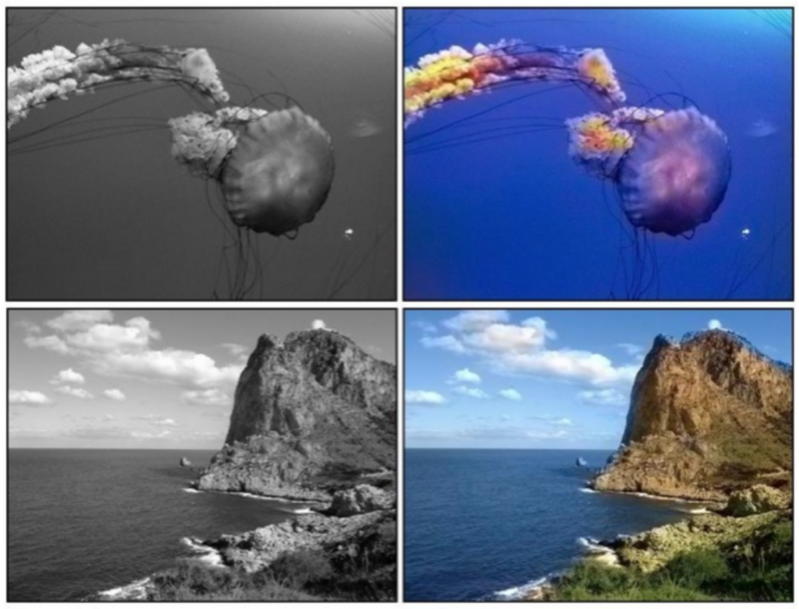
\includegraphics[height=0.8\textheight, width=\textwidth, keepaspectratio]{./images/autoencoders/image_colorization.png}
    \caption{Image colorization using Autoencoders}
\end{figure}

\end{frame}